\documentclass[letterpaper, 11pt]{article}
\usepackage{latexsym}
\usepackage{amssymb}
\usepackage{times}
%\usepackage[in]{fullpage}
\usepackage{amsmath,amsfonts,amsthm}
\usepackage{graphicx}

%\documentclass[11pt]{article}
%\pagestyle{myheadings}
%\usepackage[ruled,nothing]{algorithm}
%\usepackage{algorithmic}
%\usepackage[dvips]{epsfig,graphicx}
%\numberwithin{equation}{section}

\bibliographystyle{plain}

\newenvironment{newalgo}[2]{\begin{algorithm}

\caption{\textsc{#1}}\label{#2}

\begin{algorithmic}[1]}{\end{algorithmic}\end{algorithm}}



\newcommand{\gm}{\gamma}
\newcommand{\wh}{\widehat}
\newcommand{\rep}{representation}
\newcommand{\rv}{random variable}
\newcommand{\la}{\lambda}
\newcommand{\wt}{\widetilde}
\newcommand{\st}{such that}
\newcommand{\slvary}{slowly varying}
\newcommand{\ma}{moving average}
\newcommand{\regvary}{regularly varying}
\newcommand{\asy}{asymptotic}
\newcommand{\ts}{time series}
\newcommand{\id}{infinitely divisible}
\newcommand{\seq}{sequence}
\newcommand{\fidi}{finite dimensional \ds}

\newcommand{\ble}{\begin{lemma}}
\newcommand{\ele}{\end{lemma}}
\newcommand{\bfX}{{\bf X}}
\newcommand{\pro}{probabilit}
\newcommand{\BX}{{\bf X}}
\newcommand{\BY}{{\bf Y}}
\newcommand{\BZ}{{\bf Z}}
\newcommand{\BV}{{\bf V}}
\newcommand{\BW}{{\bf W}}
\newcommand{\reals}{{\mathbb R}}
\newcommand{\bbr}{\reals}

\newcommand{\balpha}{\mbox{\boldmath$\alpha$}}
\newcommand{\bbeta}{\mbox{\boldmath$\beta$}}
\newcommand{\bmu}{\mbox{\boldmath$\mu$}}
\newcommand{\tbmu}{\mbox{\boldmath${\tilde \mu}$}}
\newcommand{\bEta}{\mbox{\boldmath$\eta$}}


\def \br#1{\left \{#1 \right \}}
\def \pr#1{\left (#1 \right)}

\newcommand{\Gm}{\Gamma}
\newcommand{\ep}{\epsilon}


\newtheorem{lemma}{Lemma}[section]
\newtheorem{figur}[lemma]{Figure}
\newtheorem{theorem}[lemma]{Theorem}
\newtheorem{proposition}[lemma]{Proposition}
\newtheorem{definition}[lemma]{Definition}
\newtheorem{corollary}[lemma]{Corollary}
\newtheorem{example}[lemma]{Example}
\newtheorem{exercise}[lemma]{Exercise}
\newtheorem{remark}[lemma]{Remark}
\newtheorem{fig}[lemma]{Figure}
\newtheorem{tab}[lemma]{Table}
\newtheorem{fact}[lemma]{Fact}
\newtheorem{test}{Lemma}
\newtheorem{algorithm}[lemma]{Algorithm}

\newcommand{\play}{\displaystyle}

\newcommand{\ms}{measure}
\newcommand{\beao}{\begin{eqnarray*}}
\newcommand{\eeao}{\end{eqnarray*}\noindent}
\newcommand{\beam}{\begin{eqnarray}}
\newcommand{\eeam}{\end{eqnarray}\noindent}

\newcommand{\halmos}{\hfill\mbox{\qed}\\}
\newcommand{\fct}{function}
\newcommand{\ins}{insurance}
\newcommand{\ds}{distribution}

\newcommand{\one}{{\bf 1}}
\newcommand{\eid}{\buildrel{\rm d}\over {=}}
\newcommand {\Or}{\rm ORDER}
\newcommand {\In}{\rm INTER}

\newcommand{\bbd}{{\mathbb D}}
\newcommand{\vi}{$V_{ij}$ }
\newcommand{\rr}{R^{\prime\prime}}
%\newcommand{\R}{R^\prime}
\newcommand{\ci}{\frac{1}{c}}
\newcommand{\Vi}{V(n)}
\newcommand{\dR}{\mathcal R}
\newcommand{\md}[1]{\left(\ \rm{mod}\ \it{#1}\right)}
\newcommand{\So}{s}
%\begin{document}
%\def\DoubleSpace{\baselineskip=24pt}
%\DoubleSpace \sloppy

\begin{document}



\title{Parallel Programming \\ Assignment \#1: OpenMP Smoother}
\author{Yifan Ge }


\maketitle



\section{Problem 1}

Evaluate the functions \texttt{smoothSerialXY} and \texttt{smoothSerialYX} that iterate in column major and row major order respectively for kernels of size $3 \times 3$, $5 \times 5$, $7 \times 7$.

\begin{enumerate}
\item \textbf{What is the relative performance of the two functions. Give a runtime number (average of 20 trials) for both.}\\
\texttt{smoothSerialYX} show better performance over \texttt{smoothSerialXY}.
\begin{table}[h]
    \hspace{30pt}
    \begin{tabular}{|c|c|c|}
        \hline
        Running time (sec) & \texttt{smoothSerialXY} & \texttt{smoothSerialYX} \\ \hline
        $3 \times 3$          & 5.4520186             & 4.3357826             \\ 
        $5 \times 5$        & 11.9414182            & 10.8491422            \\ 
        $7 \times 7$         & 21.8240202            & 20.5165304            \\ 
        \hline
    \end{tabular}
    \caption{Performance comparison}
\end{table}
\item \textbf{Explain the performance difference.}\\
The performance difference is due to memory layout of array used in C. In C, arrays are stored in row major order. As the data stored in consecutive cache or memory spaces can be fetched at the same time, \texttt{smoothSerialYX} takes the advantage of this and these data can be used in the inner loop. While the data need in the inner loop of \texttt{smoothSerialXY} are not stored consecutively, more memory fetches are needed, and the data in the cache  need to be written back to memory more frequently. 
\end{enumerate}



\section{Problem 2}
Create a parallel for loop implementation in the function \texttt{smoothParallelYXFor}. This should consist of adding an OpenMP parallel for directive around the outer loop of \texttt{smoothSerialYX}.
\begin{enumerate}
\item \textbf{Generate speedup plots for 1, 2, 4, 8, 16 and 32 threads. You will have to specify the number of threads to run using \texttt{omp\_set\_num\_threads}.}\\
Figure \ref{fig:yxspeedup} shows the speedup for 1, 2, 4, 8, 16 and 32 threads. 
\begin{figure}[h]
    \centering
    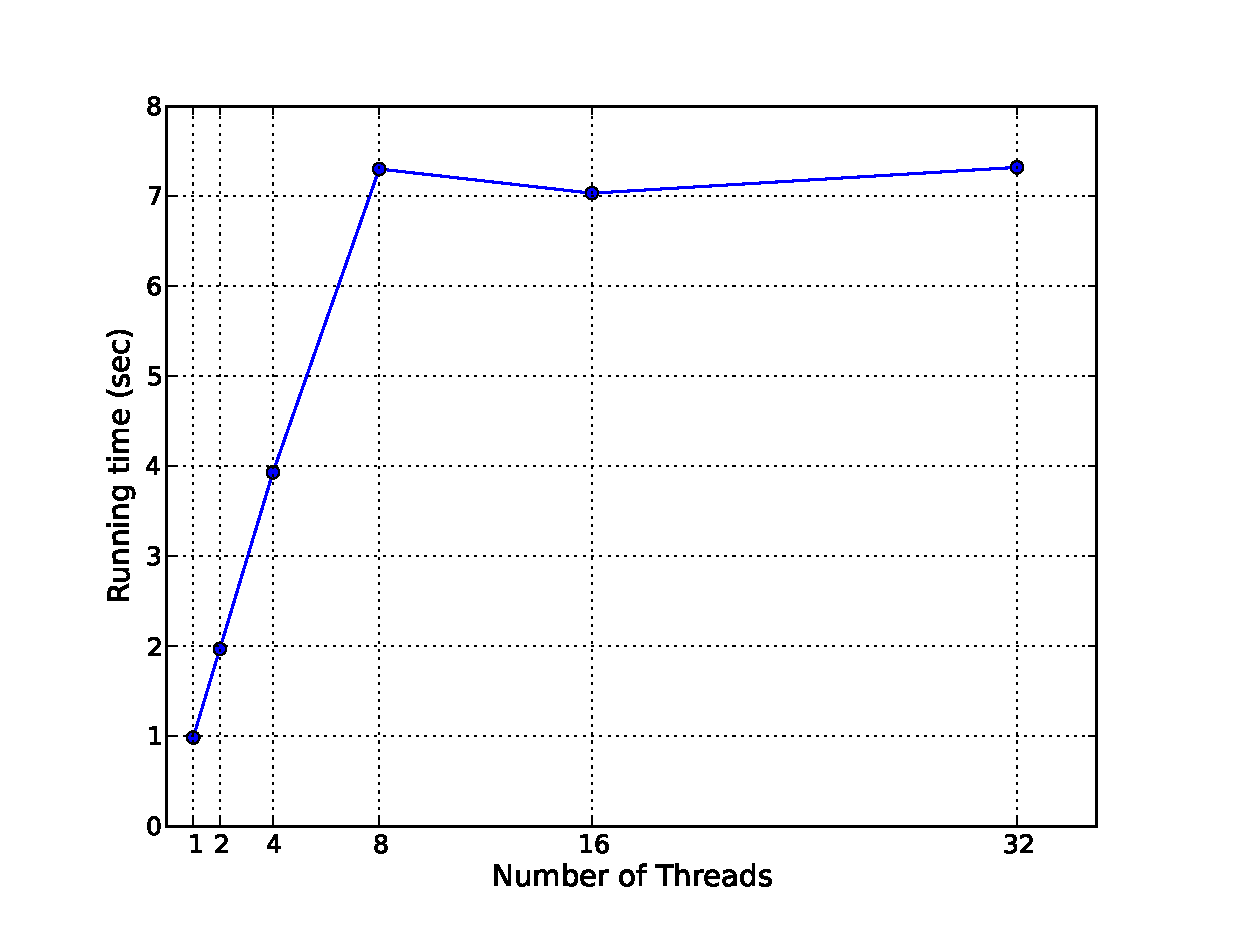
\includegraphics[width=3.8in]{yxparallelspeedup.eps}
    \caption{Speedup of \texttt{smoothSerialYX} for different number of threads}
    \label{fig:yxspeedup}
\end{figure}
\item \textbf{Describe the results. What type of speedup was realized? When did speedup tail off? Why? What hardware did this run on and how did that influence your result.}\\
With the number of threads increasing from $1$ to $8$, a linear speedup is realized. When the number of threads goes beyond $8$, the speedup begins to tail off. This is because I am running this program on a 8-core machine. The optimal number of threads is $8$. When the number of threads reaches $8$, the processors have already been fully utilized, and the speedup cannot be improved more. 

\item \textbf{Estimate the value of $P$ in Amdahl's law based on your results for $1$ to $8$ threads.}\\
For the number of threads ranging from $1$ to $8$, the result shows a linear speedup, so the value of $P$ is close to $1$. Specifically, when the number of threads equals $8$, the speedup is $7.30$. Using the equation of Amadahl's Law:\\
$$
    Speedup=\frac{1}{1-P+\frac{P}{S}}
$$
Here $Speedup=7.30$ and $S=8$, we can get $P=0.986$.
\end{enumerate}

\section{Problem 3}
Create a parallel for loop implementation in the function \texttt{smoothParallelXYFor}. This should consist of adding an OpenMP parallel for directive around the outer loop of \texttt{smoothSerialXY}.

\begin{enumerate}
\item \textbf{Generate speedup plots for 1, 2, 4 and 8 threads.}\\
Figure \ref{fig:xyspeedup} shows the speedup of \texttt{smoothParallelXYFor} for different number of threads.
\begin{figure}[h]
    \centering
    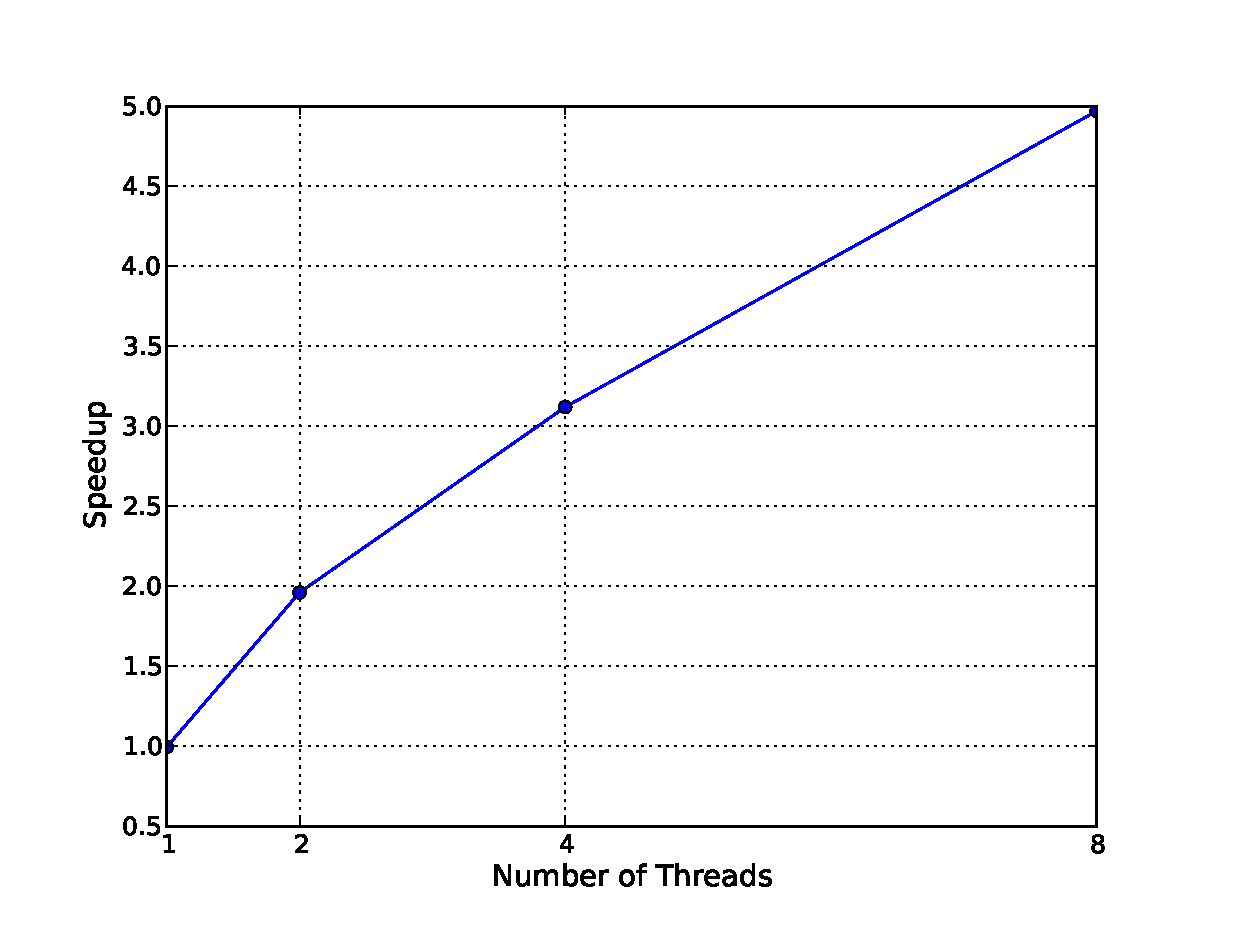
\includegraphics[width=3.8in]{xyparallelspeedup.eps}
    \caption{Speedup of \texttt{smoothParallelXYFor} for different number of threads}
    \label{fig:xyspeedup}
\end{figure}

\item \textbf{Qualitatively compare the speedup of this code to the $YX$ parallel version. Explain the differences. \textit{Note:} this question is about the relative speedup, not the relative performance of the serial versions.}\\
The speedup of \texttt{smoothParallelXYFor} is relatively lower than the speedup of \texttt{smoothParallelYXFor}. \\
As the memory spaces accessed are not consecutive in \texttt{smoothParallelXYFor}, they cannot be fetched together into the cache line. With more threads working and fetching data into the cache line, the data in the cache need to be write back to the memory more frequently than \texttt{smoothParallelYXFor}. Moreover, there is higher possibility that different threads are working on consecutive memory spaces, and this can causes more inferences which lowers the speedup.
\end{enumerate}

\section{Problem 4}
Create a function \texttt{smoothParallelForCoalesced} that coalesces the two for loops in to a single loop.
\begin{enumerate}
\item \textbf{Generate speedup plots for 1, 2, 4 and 8 threads.}
Figure \ref{fig:coalesce} shows the speedup of \texttt{smoothParallelForCoalescesd} for 1, 2, 4 and 8 threads.
\begin{figure}[h]
    \centering
    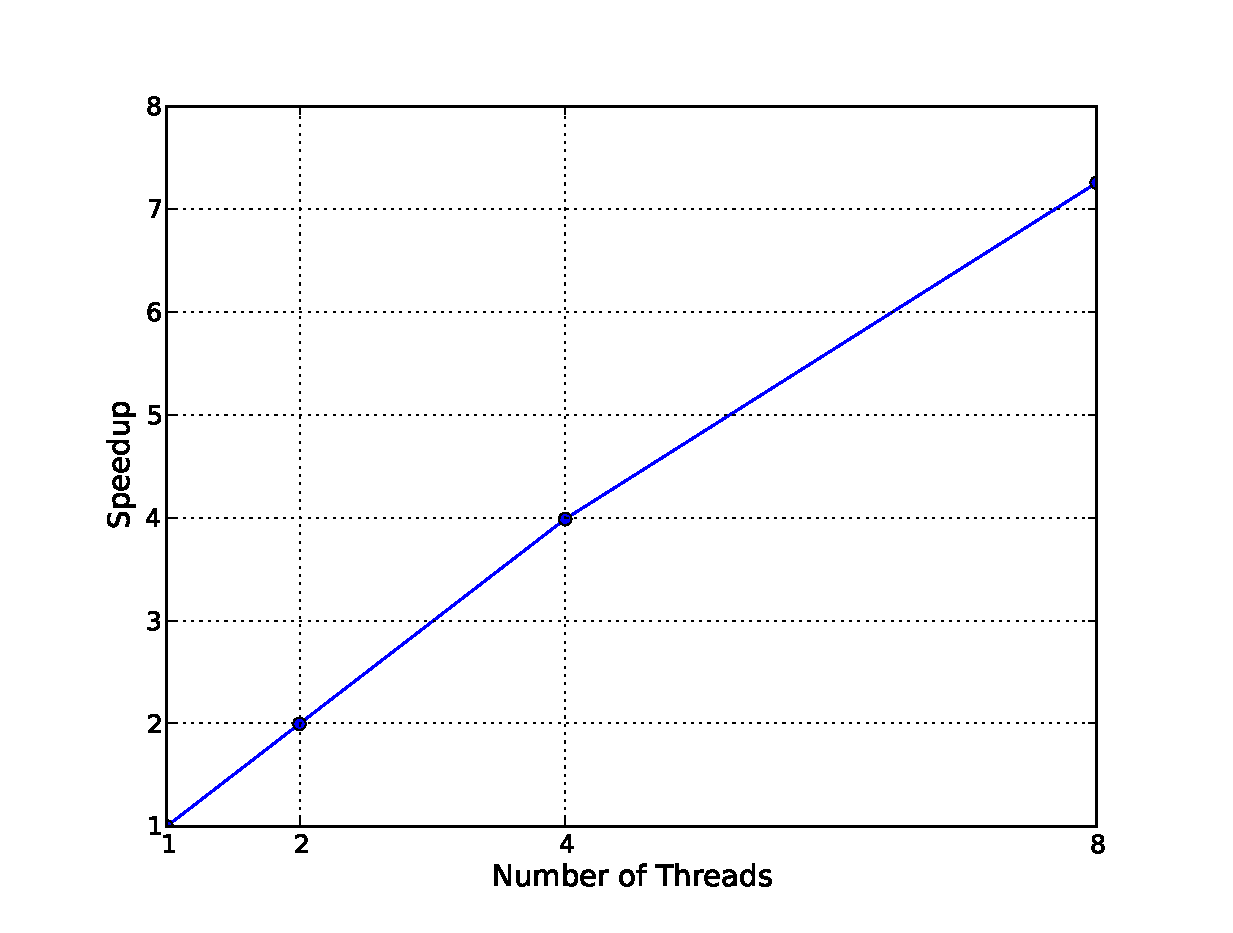
\includegraphics[width=3.8in]{coalesce.eps}
    \caption{Speedup of \texttt{smoothParallelForCoalesced}}
    \label{fig:coalesce}
\end{figure}

\item \textbf{Did coalescing the loop improve absolute performance or speedup? Explain why or why not (for both absolute performance and speedup.)}\\
No for both absolute performance and speedup. As for the absolute performance, \texttt{smoothParallelForCoalesced} uses the row major order to manipulate the array, which is no different from \texttt{smoothParallelYXFor}. So the way memory is accessed is the same, which leads to no absolute performance improvement.\\
As for the speedup, there is still no improvement. This is because we have made both \texttt{x} and \texttt{y} private in \texttt{smoothParallelYXFor} and the variables used are loop independent. So even though the loops are flattened, the ways OpenMP making the computations parallel are the same.
\end{enumerate}

\section{Problem 5}
Write and compare the following two programs for computing the smoothed value of two arrays. Program \#1 uses two invocations of \texttt{smoothParallelYXFor}. Program \#2 merges the two loops, evaluating both arrays in a single parallel OpenMP for loop.

\begin{enumerate}
\item \textbf{Generate speedup plots for 1, 2, 4 and 8 threads.}\\
Figure \ref{fig:prog1} shows the speedup of using two invocations of \texttt{smoothParallelYXFor}.  Figure \ref{fig:prog2} shows the speedup of merging the two loops. 
\begin{figure}[h]
    \centering
    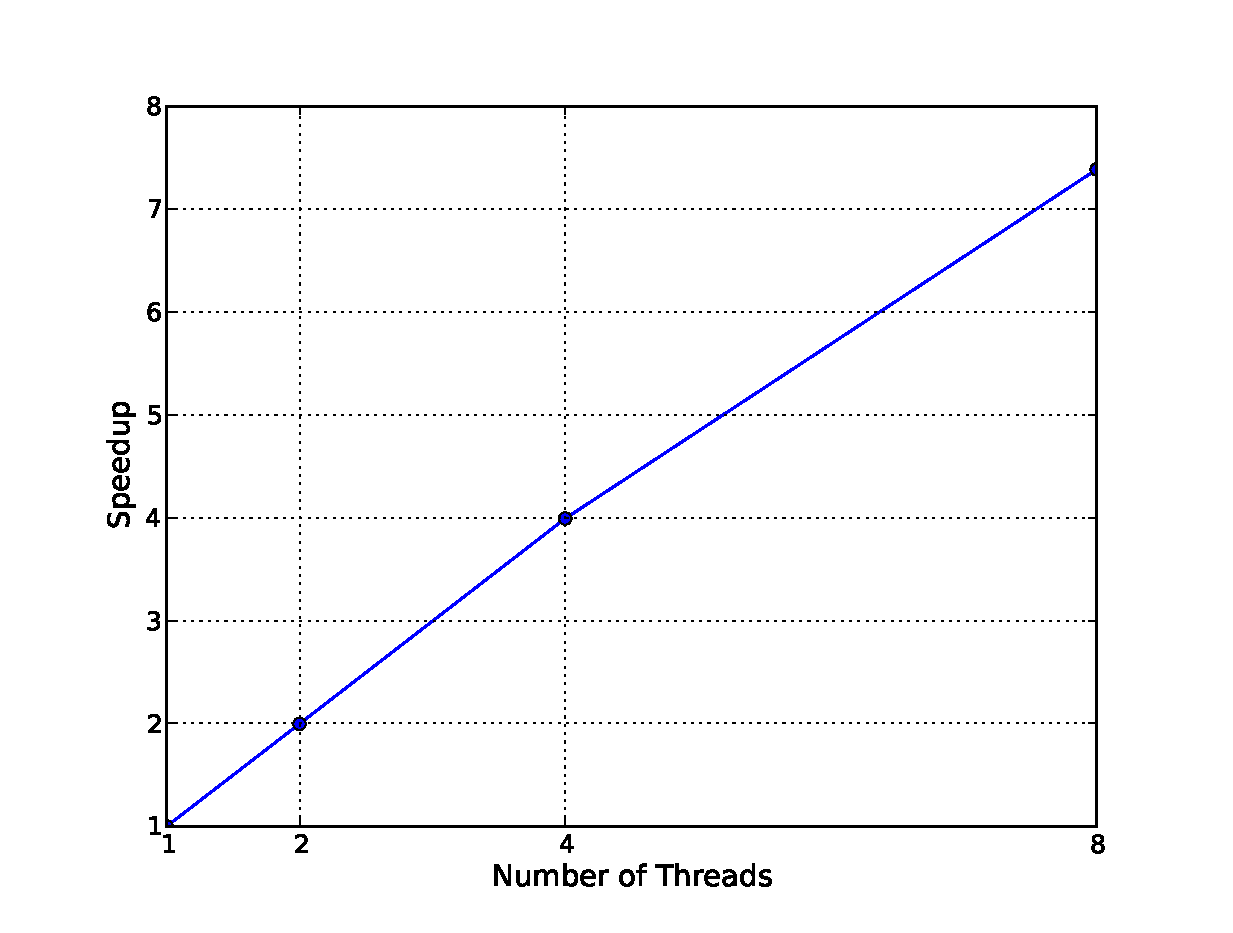
\includegraphics[width=3.8in]{twoinv.eps}
    \caption{Speedup of Program \#1}
    \label{fig:prog1}
\end{figure}

\begin{figure}[h]
    \centering
    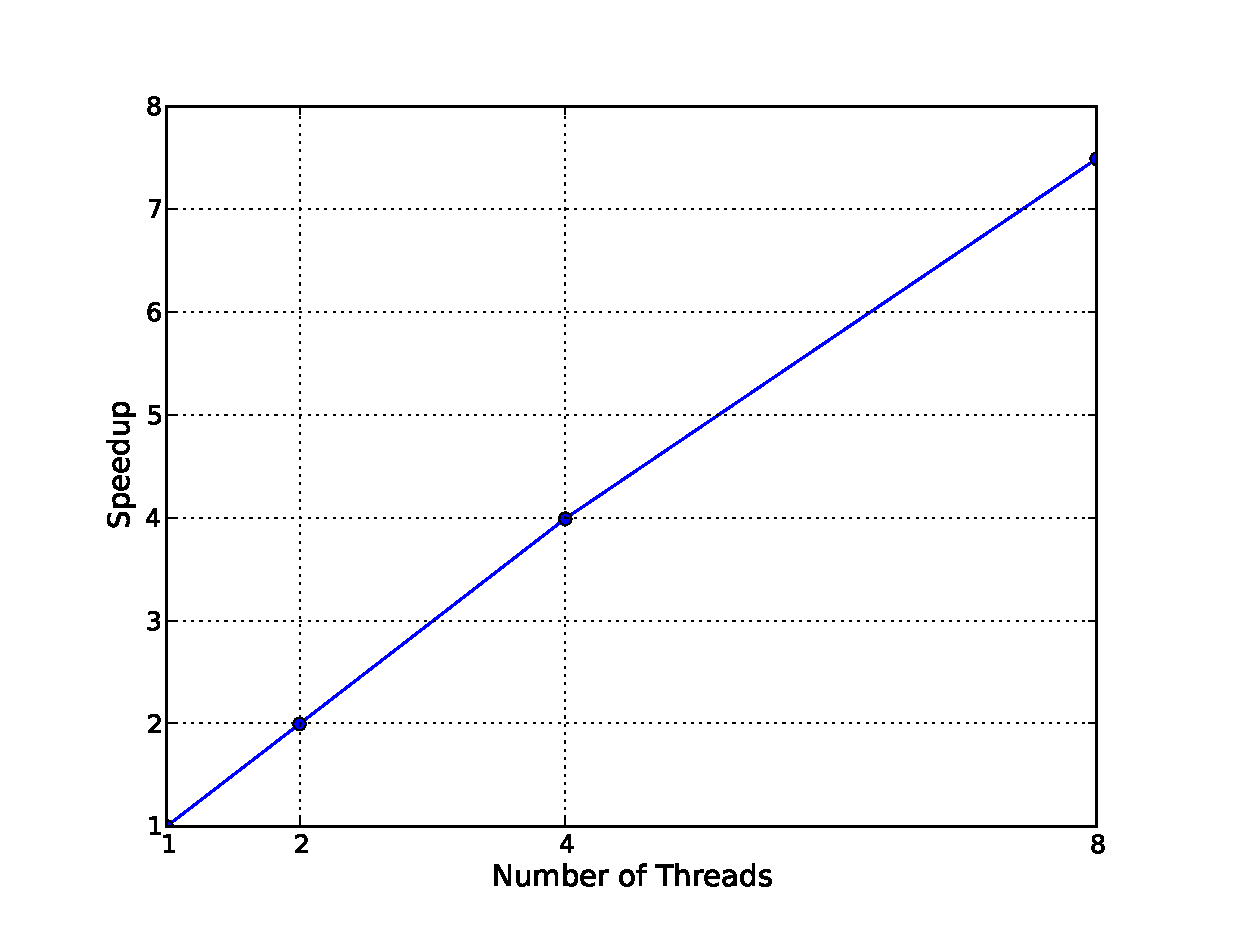
\includegraphics[width=3.8in]{merged.eps}
    \caption{Speedup of Program \#2}
    \label{fig:prog2}
\end{figure}
\item \textbf{What is the relative performance of the two programs. What benefit does loop merging have on this code? Explain why.}

\begin{table}
    \hspace{70pt}
    \begin{tabular}{|c|c|c|}
        \hline
        Running time (sec) & Program \#1 & Program \#2 \\ \hline
        Threads=1          & 22.0034534  & 21.87734    \\ 
        Threads=2          & 11.0218692  & 10.9635202  \\ 
        Threads=4          & 5.5110594   & 5.4814878   \\ 
        Threads=8          & 2.978827    & 2.9210408   \\ 
        Threads=16         & 3.0273454   & 2.9817048   \\ 
        Threads=32         & 3.0069572   & 2.9419442   \\
        \hline
    \end{tabular}
    \caption{Performance comparison of Program \#1 and Program \#2}
    \label{tab:prog12comp}
\end{table}

Table \ref{tab:prog12comp} shows the comparison of the running time of Program \#1 and Program \#2. We can see the performance of merging the two loops is relatively slightly better than invoking \texttt{smoothParallelYXFor} twice. \\
The benefits of merging the loops instead of calling the function twice are:
\begin{enumerate}
\item The intermediate results like \texttt{y * dim + x} can be reused. This reduces the cost to computing these values twice. 
\item Merging the loops can have less startup costs.
\end{enumerate}
\end{enumerate}

\end{document}




































